\documentclass{beamer}

%%% Compile flags
% Show algorithm pseudocode
\newif\ifshowalgo
\showalgotrue

% Put required libraries into library.tex
\usepackage[linesnumbered,ruled]{algorithm2e}
\usepackage{amsmath}
\usepackage{array}
\usepackage{float}
\usepackage{listings}
\usepackage{url}
\usepackage{setspace}
\usepackage{tikz}

\usetikzlibrary{arrows}
\usetikzlibrary[backgrounds]
\usetikzlibrary{calc}
\usetikzlibrary{decorations.markings}
\usetikzlibrary{fit}
\usetikzlibrary{shadows}
\usetikzlibrary{shapes.arrows}
\usetikzlibrary{shapes.geometric}



% Slide specific packages
\usepackage{adjustbox}
\usepackage{biblatex}
\usepackage{caption}
\usepackage{multicol}
\captionsetup{font=scriptsize,labelfont=scriptsize}
% if figure only 
%\captionsetup[figure]{font=scriptsize,labelfont=scriptsize}

% Your bibliography goes here
\bibliography{bibliography}

% Define styles
% Tikz figure styles
\tikzstyle{vecArrow} = [thick, decoration={markings,mark=at position
  1 with {\arrow[semithick]{open triangle 60}}},
  double distance=1.4pt, shorten >= 5.5pt, preaction = {decorate},
  postaction = {draw,line width=2pt, white,shorten >= 4.5pt}
]
\tikzstyle{component} = [draw,text centered,rounded corners,drop
  shadow,text width=8em,fill=red!20,minimum height=6em
]
\tikzstyle{dispatcher} = [component,minimum height=19.3em]
\tikzstyle{system}=[draw,dashed,rounded corners,fill=yellow!30]


% Listing styles
\lstset{
  frame=LRBT,
  basicstyle=\ttfamily\small\color{black},
  commentstyle = \ttfamily\color{blue!50},
  keywordstyle=\ttfamily\color{green},
  stringstyle=\color{red!80},
}


% Slide style setting
\usetheme{Boadilla}
\setbeamertemplate{navigation symbols}{}%remove navigation symbols

\title{Job Dispatching and Scheduling under Heterogeneous Clusters}
\author{Ting-Chou Lin}

\AtBeginSection[]{
  \begin{frame}<beamer>
    \frametitle{Outline}
    \tableofcontents[
      currentsubsection,
      sectionstyle=show/shaded,
      subsectionstyle=show/hide,
    ]
  \end{frame}
}

\begin{document}

\begin{frame}
  \titlepage
  \label{title-page}
\end{frame}
\begin{frame}
  \frametitle{Outline}
  \tableofcontents[subsectionstyle=show/hide]
\end{frame}

\section{Introduction}

\begin{frame}
  \frametitle{Background}
  \setbeamercovered{transparent}
  \begin{itemize}[<+->]
    \item As the amount of data and computing demand increases, more and
      more companies tend to build their own data centers --- Private
      Cloud.
    \item For elasticity, rather than dedicating servers for particular
      applications, more people tend to build a large cluster for all
      needs.
  \end{itemize}
\end{frame}
\begin{frame}
  \frametitle{Background --- Job Characteristics}
  \setbeamercovered{transparent}
  \begin{itemize}[<+->]
    \item In data centers, jobs come with different characteristics.
      \begin{itemize}
        \item Importance/Priority
        \item Computation resource demand
          \begin{itemize}
            \item CPU bound versus I/O bound
            \item <.-> Requires large RAM
            \item <.-> Leverage GPGPU
          \end{itemize}
        \item <.(2)->{\alert<.(2)->{Deadline/Service Level Agreement}}
      \end{itemize}
    \item Moreover, some of them should be completed before time
      constraints.
      \begin{itemize}
        \item <.-> Billing jobs should be done within days after
          charge-off.
        \item <.-> Research experiments are not that urgent.
      \end{itemize}
  \end{itemize}
\end{frame}
\begin{frame}
  \frametitle{Background --- Server Characteristics}
  \setbeamercovered{transparent}
  \begin{itemize}[<+->]
    \item Resources in data centers are usually \emph{limited} and
      \emph{fixed}
      \begin{itemize}
        \item Purchase new ones and remove obsolete ones only on
          periodic equipment upgrades.
        \item \textbf{The number of workers is fixed between upgrades.}
      \end{itemize}
    \item <.(-2)-> Servers in the cluster are \alert{heterogeneous}.
      \begin{itemize}
        \item Old servers coexist with new servers.
        \item <.-> Only few servers have special capabilities, like Giga-LAN
          or GPGPU.
      \end{itemize}
  \end{itemize}
\end{frame}
\begin{frame}
  \frametitle{Goal}
  \begin{itemize}
    \item Implement a resource management component that \emph{dynamically}
      adjusts resource for each job.
    \item System administrator can easily specify different policies to
      adapt to their needs.
    \item The system should take server \alert{heterogeneity} into consideration.
  \end{itemize}
\end{frame}
\begin{frame}
  \frametitle{Target Environment --- CHT's Data Center}
  \begin{itemize}
    \item Physical servers only +
      JPPF\footnote[frame]{\tiny\fullcite{cite:JPPF}}.
    \item Old and new servers coexists --- heterogeneous environment.
    \item Most jobs process files (billing accounting).
    \item Jobs are split into many \emph{tasks}, each can be processed
      in parallel.
    \item Data is shared via NFS.
    \item Servers may fail.
  \end{itemize}
\end{frame}


\section{System Architecture}

\begin{frame}
  \frametitle{System Architecture -- Overview}
  \begin{columns}
    \begin{column}{.5\textwidth}
      \begin{figure}
        \resizebox{\linewidth}{!}{
          \pgfdeclarelayer{background}
\pgfdeclarelayer{foreground}
\pgfsetlayers{background,main,foreground}

\begin{tikzpicture}
  \node[](management){\pgfdeclarelayer{background}
\begin{tikzpicture}
  \node[](key-comp){\input{figures/manage-compo-relation.tikz}};
  \path (key-comp.south) + (0, -0.5) node(comp-caption){Management System};
  \begin{pgfonlayer}{background}
    \node[system,fit=(key-comp) (comp-caption)]{} ;
  \end{pgfonlayer}
\end{tikzpicture}
};

  % Client
  %\coordinate (client-mid) at (management.east) + (5em,0);
  %\path (client-mid) + (0,-2) node[component,text width=5em]{Client};
  %\path (client-mid) + (0, 2) node[component,text width=5em]{Client};

  % Workers
  \coordinate (l1) at (management.south west);
  \coordinate (l2) at (management.south east);
  \path (l1) + (0, -3)
  node[component,text width=4em,minimum height=3em](w1){worker};
  \path (l2) + (0, -3)
  node[component,text width=4em,minimum height=3em](w4){worker};
  \path ($(w1)!0.33!(w4)$)
  node[component,text width=4em,minimum height=3em](w2){worker};
  \path ($(w1)!0.66!(w4)$)
  node[component,text width=4em,minimum height=3em](w3){worker};
  \draw[vecArrow] ([xshift=-5]$(l1)!0.2!(l2)$) to ([xshift=-5,yshift=3]w1.north);
  \draw[vecArrow] ([xshift=-5]$(l1)!0.4!(l2)$) to ([xshift=-5,yshift=3]w2.north);
  \draw[vecArrow] ([xshift=-5]$(l1)!0.6!(l2)$) to ([xshift=-5,yshift=3]w3.north);
  \draw[vecArrow] ([xshift=-5]$(l1)!0.8!(l2)$) to ([xshift=-5,yshift=3]w4.north);
  \draw[vecArrow] ([xshift=5,yshift=3]w1.north) to ([xshift=5]$(l1)!0.2!(l2)$);
  \draw[vecArrow] ([xshift=5,yshift=3]w2.north) to ([xshift=5]$(l1)!0.4!(l2)$);
  \draw[vecArrow] ([xshift=5,yshift=3]w3.north) to ([xshift=5]$(l1)!0.6!(l2)$);
  \draw[vecArrow] ([xshift=5,yshift=3]w4.north) to ([xshift=5]$(l1)!0.8!(l2)$);
\end{tikzpicture}


        }
        \caption{Architecture Overview}
        \label{fig:archi-overview}
      \end{figure}
    \end{column}
    \begin{column}{.5\textwidth}
      \begin{itemize}
        \item Each component is a RPC server
        \item As a cluster management system or extension
          components of existent cloud systems
      \end{itemize}
    \end{column}
  \end{columns}
\end{frame}

\begin{frame}
  \frametitle{System Architecture -- Client}
  \only<1>{
    \begin{itemize}
      \item The programming interface users sends jobs to the system for execution
      \item Users can specify attributes for jobs
        \begin{itemize}
          \item Deadline
          \item Priority
          \item \ldots
        \end{itemize}
      \item Supports background execution

    \end{itemize}
  }
  \only<2>{
    \newfloat{Example Code}{H}{myc}
    \begin{Example Code}
      \lstset{
        frame=LRBT,
        basicstyle=\ttfamily\tiny\color{black},
        commentstyle = \ttfamily\color{blue!50},
        keywordstyle=\ttfamily\color{green},
        stringstyle=\color{red!80},
      }
      \begin{lstlisting}[language=Ruby]
  client = Client.new
  client.register(SERVER_ADDRESS)
  client.start
  j1 = Job.new('Job1')
  j1.add_task Task.new(...)
  ... # Add more tasks
  j2 = Job.new('Job2')
  j2.add_task Task.new(...)
  ... # Add more tasks
  # 200-second deadline
  j1.deadline = j2.deadline = Time.now + 200.0
  # Submit j1 and j2 together
  # Background execution
  j12_waiter = client.submit_job([j1,j2])
  # Do other time consuming computation
  ...
  j3 = Job.new('Job3')
  j3.add_task Task.new(...)
  ... # Add more tasks
  # Remaining part can't run until j3 is done
  j3_waiter = client.submit_job(j3)
  client.wait(j3_waiter)
  # Some more things to do
  ...
  # Wait until j1 and j2 is done.
  client.wait(j12_waiter)
  # Combning j1, j2 and j3
  ...
\end{lstlisting}

      \caption{Sample code of client usage}
    \end{Example Code}
  }
\end{frame}

\begin{frame}
  \frametitle{System Architecture -- Worker}
  % TODO Hurray!!!!!! I like this part!!!!!
\end{frame}

\begin{frame}
  \frametitle{System Architecture -- Decision Maker}
  % TODO Hurray!!!!!! I like this part!!!!!
\end{frame}

\begin{frame}
  \frametitle{System Architecture -- Status Checker}
  % TODO Hurray!!!!!! I like this part!!!!!
\end{frame}

\begin{frame}
  \frametitle{System Architecture -- Dispatcher}
  % TODO Hurray!!!!!! I like this part!!!!!
\end{frame}

\begin{frame}
  \frametitle{Work flow -- Standalone Mode}
\end{frame}

\begin{frame}
  \frametitle{Work flow -- Case study: Integration with JPPF}
  \begin{itemize}[<+->]
      \only<1-2>{
      \item JPPF (Java Parallel Processing Framework) is a very popular open-source cluster management
        framework
        \begin{itemize}
          \item <.->Very easy to deploy
          \item <.->GUI monitoring tools
          \item <.->Active development
        \end{itemize}
      \item Doesn't support \emph{centralized} and
        \emph{node-aware} scheduling
      }
      \only<3->{
      \item Provides API for jobs set "filters" for a job -- to reject a
        node of from running that job
      \item Leveraging this API, we can somehow implement node-aware
        scheduling by \pause
        \begin{enumerate}
          \item Contact the system for scheduling information
          \item Get scheduled worker of the job
          \item Reject if this node is not scheduled
        \end{enumerate}
      }
  \end{itemize}
\end{frame}


\section{Work Flow}
\begin{frame}
  \frametitle{Work Flow -- Job Submission}
  \begin{enumerate}
    \item Client submits a job batch to dispatcher.
    \item Dispatcher passes information to decision maker for a new
      schedule.
    \item Decision maker obtains required information from status
      checker and schedules.
    \item Dispatcher updates job-worker relationship table according to
      the new schedule.
  \end{enumerate}
\end{frame}
\begin{frame}
  \frametitle{Work Flow -- Task Execution}
  \only<1>{
    \begin{enumerate}
      \item Client forks a task thread and notifies dispatcher a task is
        ready to run.
      \item The task thread waits for an available worker. This is a
        blocking operation.
      \item After the task thread obtains a worker, client forks another
        task thread and goes 2.
    \end{enumerate}
  }

  \only<2>{
    \begin{enumerate}
      \setcounter{enumi}{3}
      \item Client thread contacts the assigned worker and sends
        required information about the task: command, parameters, etc.
      \item Tells the worker to run the task and waits for the result.
        This is also a blocking call.
      \item After obtaining the result, client remove the task from the
        remaining task list and notifies the dispatcher to release the
        worker.
      \item Dispatcher assigns the released worker to next job
        according to the current schedule plan.
    \end{enumerate}
  }
\end{frame}
\begin{frame}
  \frametitle{Work Flow -- Job Completion}
  \begin{enumerate}
    \item After the last task of a job finished, notifies dispatcher to
      remove a job.
    \item Dispatcher removes the job entry and reschedules.
  \end{enumerate}
\end{frame}
\begin{frame}
  \frametitle{Work Flow -- Monitoring}
  \begin{enumerate}
    \item Status checker periodically pings each worker for its status.
    \item Also on each ping, collects execution statistics.
    \item If a worker stucks at occupied status for too long, forcibly
      releases it.
    \item If it found servers fail or recover from failure, tells the
      dispatcher to update the schedule.
  \end{enumerate}
\end{frame}
\begin{frame}
  \frametitle{Rescheduling Conditions}
  \begin{itemize}
    \item Job change
    \item Worker change
  \end{itemize}
\end{frame}

\section{Policy}

\begin{frame}
  \frametitle{Policy}
  \begin{itemize}
    \item The scheduling algorithm used by the system.
    \item Each of them requires different parameters.
      \begin{itemize}
        \item Provide by user 
        \item System statistics
      \end{itemize}
    \item Administrators can select different policies to fit their
      need.
  \end{itemize}
\end{frame}
\begin{frame}
  \frametitle{Outline}
  \tableofcontents[
    currentsubsection,
    sectionstyle=show/shaded,
    subsectionstyle=show/show/hide,
  ]
\end{frame}
\subsection{Priority-based}

\begin{frame}
  \frametitle{Policy -- Priority-based}
  %TODO for different needs, use different policies
  %If no deadline, only priority is specified. e.g., research experiment
  \only<1>{
    \begin{itemize}
      \item Finish the job with highest priority as fast as possible.
      \item Preserve workers to relieve starvation of low priority ones.
      \item Only priority is considered.
      \item Good for those facility whose applications do not have 
        hard time limit, such as research experiment.
    \end{itemize}
  }
  \ifshowalgo\only<2>{\scriptsize
    \resizebox{.9\textwidth}{!}{
      \begin{algorithm}[H]
        \DontPrintSemicolon % Some LaTeX compilers require you to use
        \KwIn{
  $workerSet=\{w_1, w_2, \ldots, w_m\}$,
  $jobSet=\{j_1, j_2, \ldots, j_n\}$,
  preserving rate $r\in[0,1]$
}
\KwOut{A mapping of each job to scheduled workers}
$result \gets$
KeyValueMap(key $\to \{\}$ for all key $\in jobSet$)\;
$jobSet \gets$ $sortByPriority(jobSet)$\;
$c \gets$ $min(jobSet[0]$.totalTask, $workerSet$.size$-floor((1-r) *
workerSet.$size$)$\;
$result[jobSet[0]] \gets$ $\{w_1, ..., w_c\}$\;
\For{$i=1$ to $min(m-c, n)$}{
  $result[jobSet[i]]$ $\gets$ $\{w_{c+i}\}$\;
}
\Return{result}\;


        \caption{Priority-based policy}
        \label{algo:priority-based}
      \end{algorithm}
    }
  }\fi
\end{frame}

\subsection{Proportion-based}
\begin{frame}
  \frametitle{Policy -- Proportion-based}
  %For streaming jobs, workloads may varies: For streaming jobs dependent on
  %others, if they don't have anything to process, its workload is low
  %so no workers needed, but as results come out, we should give it
  %servers
  \only<1>{
    \begin{itemize}
      \item Allocate resource proportionally according to workload 
      \item "Fair-share scheduling"~\footnote[frame]{\tiny\fullcite{cite:fair-share-scheduling}}
      \item Good for streaming jobs or jobs with dependency
    \end{itemize}
  }
  \ifshowalgo\only<2>{\scriptsize
    \resizebox{.9\textwidth}{!}{
      \begin{algorithm}[H]
        \DontPrintSemicolon % Some LaTeX compilers require you to use
        \KwIn{
  $workerSet=\{w_1, w_2, \ldots, w_m\}$,
  $jobSet=\{j_1, j_2, \ldots, j_n\}$,
}
\KwOut{A mapping of each job to scheduled workers}
$result \gets$ KeyValueMap(key $\to \{\}$ for all key $\in$
$jobSet$)\;
$jobSet \gets$ $sortByPriority(jobSet)$\;
\For{$i=1$ to $m$}{
  break if $workerSet$.size equals to 0 \;
  $c \gets$
  $min(ceil(\frac{jobSet[i].\text{workload}}{\text{total
  workload}})), workerSet.\text{size})$ \;
  $result[jobSet[i]] \gets \{\text{first $c$ element of
  $workerSet$}\}$\;
  $workerSet \setminus result[jobSet[i]]$\;
}
\Return{result}\;

        \caption{Proportion-based policy}
        \label{algo:proportion-based}
      \end{algorithm}
    }
  }\fi
\end{frame}

\subsection{Workload-based}
\begin{frame}
  \frametitle{Policy -- Workload-based}
  \only<1>{
    \begin{itemize}
      \item Consider both priority and workload
      \item Give just enough resource to meet the requirement 
      \item Achieve \emph{heterogeneity aware}allocation by always allocating
        workers that run the job the fastest
    \end{itemize}
  }
  \ifshowalgo\only<2>{\scriptsize
    \resizebox{.9\textwidth}{!}{
      \begin{algorithm}[H]
        \DontPrintSemicolon % Some LaTeX compilers require you to use
        \KwIn{
  $workerSet=\{w_1, w_2, \ldots, w_m\}$,
  $jobSet=\{j_1, j_2, \ldots, j_n\}$,
}
\KwOut{A mapping of each job to scheduled workers}
$result \gets$
KeyValueMap(key $\to \{\}$ for all key $\in jobSet$)\;
$jobSet \gets$ $sortByPriority(jobSet)$\;
\For{each job $j \in jobSet$}{
  \If{$workerSet$ is empty}{\textbf{break}\;}
  $cmp \gets function(w)$\{\Return $w$.throughput$[j]\}$\;
  $workerSet \gets$ $sort(workerSet,cmp,ACSENDING)$\;
  $i \gets 0$\;
  $throughput \gets 0$\;
  %\For{$i = 0 $ to $workerSet$.size-1}{
  %  $throughput \mathrel{+}= workerSet[i].throughput[j]$\;
  %  \If{$throughput \geq j$.workload}{
  %    \textbf{break}\;
  %  }
  %}
  \For{$i = 0$ ;\\
    $i<workerSet$.size \textbf{AND}
    $throughput < j$.workload;
    $i\mathrel{+}\mathrel{+}$
  }{
    $throughput \mathrel{+}= workerSet[i].throughput[j]$\;
  }
  $result[j] \gets workerSet[0...i]$\;
  $workerSet$.remove(0,$i$)
}

\Return{result}\;

        \caption{Workload-based policy}
        \label{algo:workload-based}
      \end{algorithm}
    }
  }\fi
\end{frame}

\subsection{Deadline-based}

\begin{frame}
  \frametitle{Policy -- Deadline-based}
  %TODO Tell this is the main focus of CHT's request, so our experiments
  %focus on this
  \only<1>{
    \begin{itemize}
      \item Scenario: billing accounting
      \item Use deadlines to estimated required workload and apply
        the workload-based policy
      \item Allocate resource just enough to meet deadlines
      \item \emph{Heterogeneity} aware scheduling
    \end{itemize}
  }
  \ifshowalgo\only<2>{\scriptsize
    \resizebox{.9\textwidth}{!}{
      \begin{algorithm}[H]
        \DontPrintSemicolon % Some LaTeX compilers require you to use
        \KwIn{
  $workerSet=\{w_1, w_2, \ldots, w_m\}$,
  $jobSet=\{j_1, j_2, \ldots, j_n\}$,
}
\KwOut{A mapping of each job to scheduled workers}
$result \gets$
KeyValueMap(key $\to \{\}$ for all key $\in jobSet$)\;
$jobSet \gets$ $sortByPriority(jobSet)$\;
\For{each job $j_i=(d_i,p_i,n_i)  \in jobSet$}{
  \If{$workerSet$ is empty}{\textbf{break}\;}
  $cmp \gets function(w)$\{\Return $1/w.execTime[j_i]\}$\;
  $workerSet \gets$ $sort(workerSet,cmp,DECSENDING)$\;
  $th \gets 0$\;
  \For{\textbf{(} $k = 0$ ;\\
    $k<workerSet$.size \textbf{AND}
    $k<n_i$ \textbf{AND}
    $th < 1/w_i.execTime[j_i]$;
    $k \gets k+1 $\textbf{)}
  }{
    $th \mathrel{+}= 1/workerSet[k].execTime[j_i]$\;
  }
  $result[j_i] \gets workerSet[0...i]$\;
  $workerSet$.remove(0,$k$)
}
assign remaining workers to jobs still in need\;
\Return{result}\;

        \caption{Deadline-based policy}
        \label{algo:deadline-based}
      \end{algorithm}
    }
  }\fi
\end{frame}


\section{Implementation}
\subsection{RPC Server Design}
\begin{frame}
  \frametitle{RPC Server Design}
  We implement all the components in our system as RPC servers.
  \begin{itemize}
    \item Lowers coupling between components.
    \item Enables changing configurations or upgrading the system
      without halting the system.
    \item Roystonea\footnote[frame]{\tiny\fullcite{cite:roystonea}}
      benefits from this design, too.
  \end{itemize}
\end{frame}
\subsection{Message Service}
\begin{frame}
  \frametitle{Message Service}
  Under traditional client-server model, server cannot actively push
  message to clients.
  \begin{itemize}
    \item Sometimes the management system needs so.
      e.g. Notifying task completion
    \item Maintaining long-last socket connection is too expensive and
      may easily reach system limit.
  \end{itemize}
  We built an underlying message pushing service.
  \begin{itemize}
    \item For each client, dispatcher maintains a message queue.
    \item Clients use long-polling\footnote[frame]{\tiny\fullcite{cite:push-pull}} to get message.
      \begin{itemize}
        \item "Long connection, slow heartbeat"
        \item Technique adopted by modern mobile message pushing services
          \footnote[frame]{\tiny\fullcite{cite:gcm}}~\footnote[frame]{\tiny\fullcite{cite:apns}}.
      \end{itemize}
  \end{itemize}
\end{frame}
\subsection{Task Queuing}
\begin{frame}
  \frametitle{Task Queuing}
  \begin{itemize}
    \item Workers are occupied until all tasks of the assigned job are
      done.
    \item Trailing idle workers.
    \item Maintain a available worker queue for each job.
    \item Enables releasing trailing idle workers earlier.
  \end{itemize}
\end{frame}

\begin{frame}
  \frametitle{Trailing Idle Worker}

  \begin{figure}[h]
    \centering
    \resizebox{\textheight}{!}{
      \pgfdeclarelayer{background}
\pgfsetlayers{background,main}
\begin{tikzpicture}
  \matrix (wmtrx2)[worker-matrix]{
    \node(w0_)[fill=red!15]{$w_0$};& \node(i1)[invisible]{};& \node(w0_)[fill=red!15]{$w_0$};&	\node(j1)[invisible]{};&	\node(w0_)[fill=red!15]{$w_0$};\\
    \node(w1_)[fill=red!15]{$w_1$};& \node(i2)[invisible]{};& \node(w1_)[fill=red!15]{$w_1$};&	\node(j2)[invisible]{};&	\node(w1_)[fill=red!15]{$w_1$};\\
    \node(w2_)[fill=red!15]{$w_2$};& \node(i3)[invisible]{};& \node(w2_)[fill=red!15]{$w_2$};&	\node(j3)[invisible]{};&	\node(w2_){$w_2$};\\
    \node(w3_)[fill=red!15]{$w_3$};& \node(i4)[invisible]{};& \node(w3_)[fill=red!15]{$w_3$};&	\node(j4)[invisible]{};&	\node(w3_){$w_3$};\\
  };
  \node[fit=(i1) (i4)]{};
  \node[fit=(j1) (j4)]{};
\end{tikzpicture}

    }
    \caption{Trailing Idle Worker}
  \end{figure}
\end{frame}

\subsection{Adaptive Adjustment}
\begin{frame}
  \frametitle{Adaptive Adjustment}
  \setbeamercovered{transparent}
  \only<1-5>{
    \begin{itemize}[<+->]
      \item We assumed that the execution time of each task can be
        predicted or obtained by profiling.
      \item <.->But accurate information is not always available.
        \begin{itemize}
          \item New applications
          \item Profiling error
          \item Machine performance degradation
        \end{itemize}
      \item Log the execution progress of each task and use it to
        estimate task execution speed
    \end{itemize}
  }
  \only<6>{
    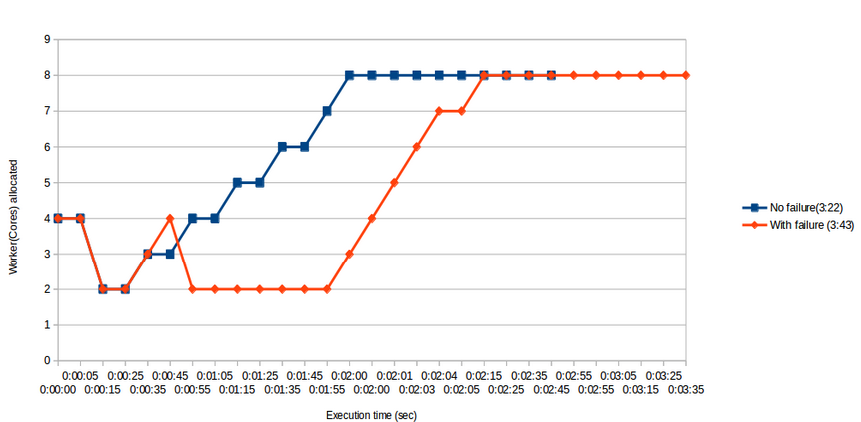
\includegraphics[width=\textwidth]{figures/adaptive.png}
  }
\end{frame}
\begin{frame}
  \frametitle{Adaptive Adjustment (Cont'd)}
  \setbeamercovered{transparent}
  \begin{itemize}
    \item Improves fault tolerance.
      \begin{itemize}
        \item Detects worker failure and assign failed task to another
          worker.
      \end{itemize}
    \item Implies we can scheduling without considering reserving resource.
      \begin{itemize}
        \item When high priority jobs arrive, kill some lower priority
          ones and gives the resource to high priority ones.  Killed
          ones we be automatically redo when there is available
          resource.
        \item In our experiment, gives about \alert{3x} throughput.
      \end{itemize}
  \end{itemize}
\end{frame}

%\subsection{Case Study: Integration with JPPF}
%\begin{frame}
%  \frametitle{Case Study: Integration with JPPF}
%  \only<1>{
%    \begin{itemize}
%      \item JPPF\footnote[frame]{\tiny\fullcite{cite:JPPF}} is a very
%        popular open-source cluster management framework.
%        \begin{itemize}
%          \item Very easy to deploy
%          \item GUI monitoring tools
%          \item Active development
%        \end{itemize}
%      \item Used in CHT's cluster.
%      \item Doesn't support \emph{centralized} and
%        \emph{node-aware} scheduling
%    \end{itemize}
%  }
%  \only<2->{
%    \begin{itemize}[<+->]
%      \item Provides API for jobs set "filters" for a job --- to reject a
%        node from running that job
%      \item<.-> Leveraging this API, we can somehow implement node-aware
%        scheduling by
%        \pause
%        \begin{enumerate}
%          \item Contact the system for scheduling information
%          \item Get scheduled worker of the job
%          \item Reject if this node is not scheduled
%        \end{enumerate}
%    \end{itemize}
%  }
%\end{frame}

\section{Experiment}
\subsection{Simulation Settings}
\begin{frame}
  \frametitle{Experiment Settings}
  \only<1>{
    Hardware
    \begin{itemize}
      \item Intel Core i5 3570 (2C4T)
      \item 16GB RAM
      \item Ubuntu 14.04 LTS
      \item Ruby 2.1.1
    \end{itemize}
  }

  \only<2>{
    Sleep-based simulation
    \begin{itemize}
      \item Sample from obtained data center logs.
      \item Take allocated CPUs as task amount and assign random numbers
        as job priorities.
      \item Sleep according to the execution time.
      \item 20 worker instances used.
    \end{itemize}
  }

  \only<3>{
    Homogeneous Environment
    \begin{itemize}
      \item Tasks in a job has identical sleep time.
      \item Each worker simply sleeps the time hold by that task.
    \end{itemize}

    Heterogeneous Environment
    \begin{itemize}

      \item Each worker will sleep an randomized additional period
        related to a worker parameter.
      \item Specify different parameter to represent different computing
        speed.
      \item Pick 1/20 of the task as GPU task and 4 out of 20 workers as
        GPU server.  When GPU task is send to a GPU worker, its sleep
        time is reduced to 1/10.
    \end{itemize}

  }
\end{frame}

\subsection{Homogeneous}
\begin{frame}
  \frametitle{Experiment Results --- Homogeneous}
  \begin{figure}[htbp]
    \centering
    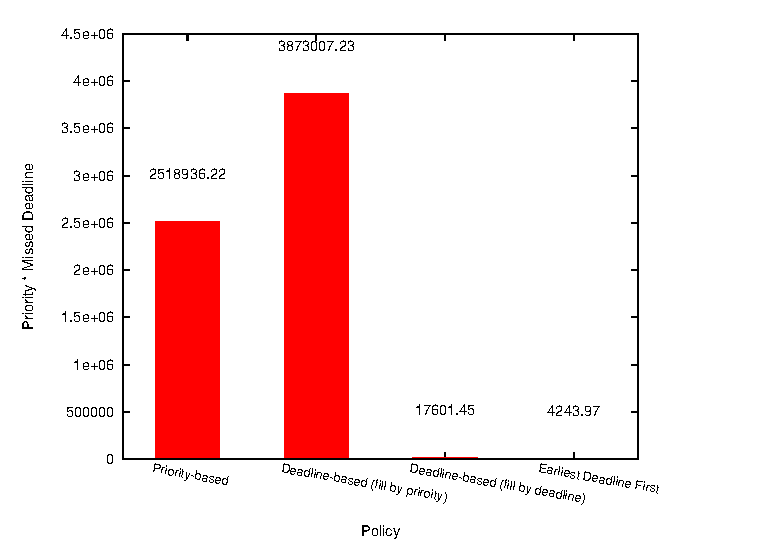
\includegraphics[width=\textwidth,height=0.7\textheight,keepaspectratio]{figures/homo.eps}
    \caption{Homogeneous Environment Setting}
  \end{figure}
\end{frame}



\end{document}
